\chapter{Задание \textnumero1}

\section{Условие}

Написать приложение по модели клиент-сервер, демонстрирующее взаимодействие параллельных процессов на отдельном компьютере с использованием сокетов в файловом пространстве имен: семейство~--- AF\_UNIX, тип~--- SOCK\_DGRAM\@. При демонстрации работы программного комплекса необходимо запустить несколько клиентов (не меньше 5) и продемонстрировать, что сервер обрабатывает обращения каждого запущенного клиента.

\section{Реализация}

Сокеты, входящие в домен AF\_UNIX используют имя сокет-файла в качестве адреса. Программа-сервер создает сокет при помощи функции socket с параметрами AF\_UNIX и SOCK\_DGRAM\@. Далее функция bind привязывает сокет к локальному адресу. После этого при помощи системного вызова recvfrom происходит блокировка процесса-сервера в ожидании сообщения от одного из процессов-клиентов. Текст программы-сервера приведён в листинге~\ref{lst:fserver}.

\begin{lstlisting}[caption={Текст программы-сервера},label=lst:fserver]
#include <stdio.h>
#include <errno.h>
#include <stdlib.h>
#include <string.h>
#include <unistd.h>
#include <signal.h>
#include <sys/types.h>
#include <sys/socket.h>

#define SOCKET_NAME "socket.soc"

int socket_fd;

void sigint_handler(int signum);

int main(void)
{
    int bytes;
    char buf[BUFSIZ];
    struct sockaddr server_name;

    if (signal(SIGINT, &sigint_handler) == SIG_ERR)
    {
        fprintf(stderr, "%s: %s\n", "signal sigint", strerror(errno));
        exit(1);
    }

    if ((socket_fd = socket(AF_UNIX, SOCK_DGRAM, 0)) < 0)
    {
        fprintf(stderr, "%s: %s\n", "socket", strerror(errno));
        exit(1);
    }

    server_name.sa_family = AF_UNIX;
    strcpy(server_name.sa_data, SOCKET_NAME);

    if (bind(socket_fd, &server_name, sizeof(server_name.sa_family) +
                                      strlen(server_name.sa_data) + 1) < 0)
    {
        fprintf(stderr, "%s: %s\n", "socket", strerror(errno));
        exit(1);
    }

    for(;;)
    {
        bytes = recvfrom(socket_fd, buf, sizeof(buf), 0, NULL, NULL);

        if (bytes < 0)
        {
            fprintf(stderr, "%s: %s\n", "recvfrom", strerror(errno));
            exit(1);
        }

        buf[bytes] = 0;
        printf("%s", buf);
    }
}

void sigint_handler(int signum)
{
    if (close(socket_fd) != 0)
    {
        fprintf(stderr, "%s: %s\n", "close socket_fd", strerror(errno));
        exit(1);
    }

    if (unlink(SOCKET_NAME) != 0)
    {
        fprintf(stderr, "%s: %s\n",
                "unlink " SOCKET_NAME, strerror(errno));
        exit(1);
    }

    exit(0);
}
\end{lstlisting}

Программа-клиент создает сокет с такими же параметрами, как и программа-сервер. Далее она задаёт тип домена и имя сокет-файла в структурe sockaddr. Отправка сообщения процессу-серверу происходит при помощи функции sendto. Текст программы-клиента приведён в листинге~\ref{lst:fclient}.

\begin{lstlisting}[caption={Текст программы-клиента},label=lst:fclient]
#include <errno.h>
#include <stdio.h>
#include <string.h>
#include <stdlib.h>
#include <unistd.h>
#include <sys/types.h>
#include <sys/socket.h>

#define SERVER_SOCKET_NAME "socket.soc"

static inline int get_input(char *buf, size_t len);

int main(void)
{
    int socket_fd;
    char buf[BUFSIZ];
    char input[BUFSIZ];
    struct sockaddr server_name;

    if ((socket_fd = socket(AF_UNIX, SOCK_DGRAM, 0)) < 0)
    {
        fprintf(stderr, "%s: %s\n", "signal sigint", strerror(errno));
        exit(1);
    }

    server_name.sa_family = AF_UNIX;
    strcpy(server_name.sa_data, SERVER_SOCKET_NAME);

    while (get_input(input, sizeof(input)))
    {
        snprintf(buf, sizeof(buf), "Client (pid %d): %s", getpid(), input);
        sendto(socket_fd, buf, strlen(buf), 0, &server_name,
               sizeof(server_name.sa_family) +
               strlen(server_name.sa_data) + 1);
    }

    if (close(socket_fd) != 0)
    {
        fprintf(stderr, "%s: %s\n", "close socket_fd", strerror(errno));
        exit(1);
    }

    return 0;
}

static inline int get_input(char *buf, size_t len)
{
    printf("> ");
    fgets(buf, len, stdin);

    return !feof(stdin);
}
\end{lstlisting}

\section{Пример работы}

На рисунке~\ref{img:task01} изображён пример работы реализованных программ.

\begin{figure}[H]
    \centering
    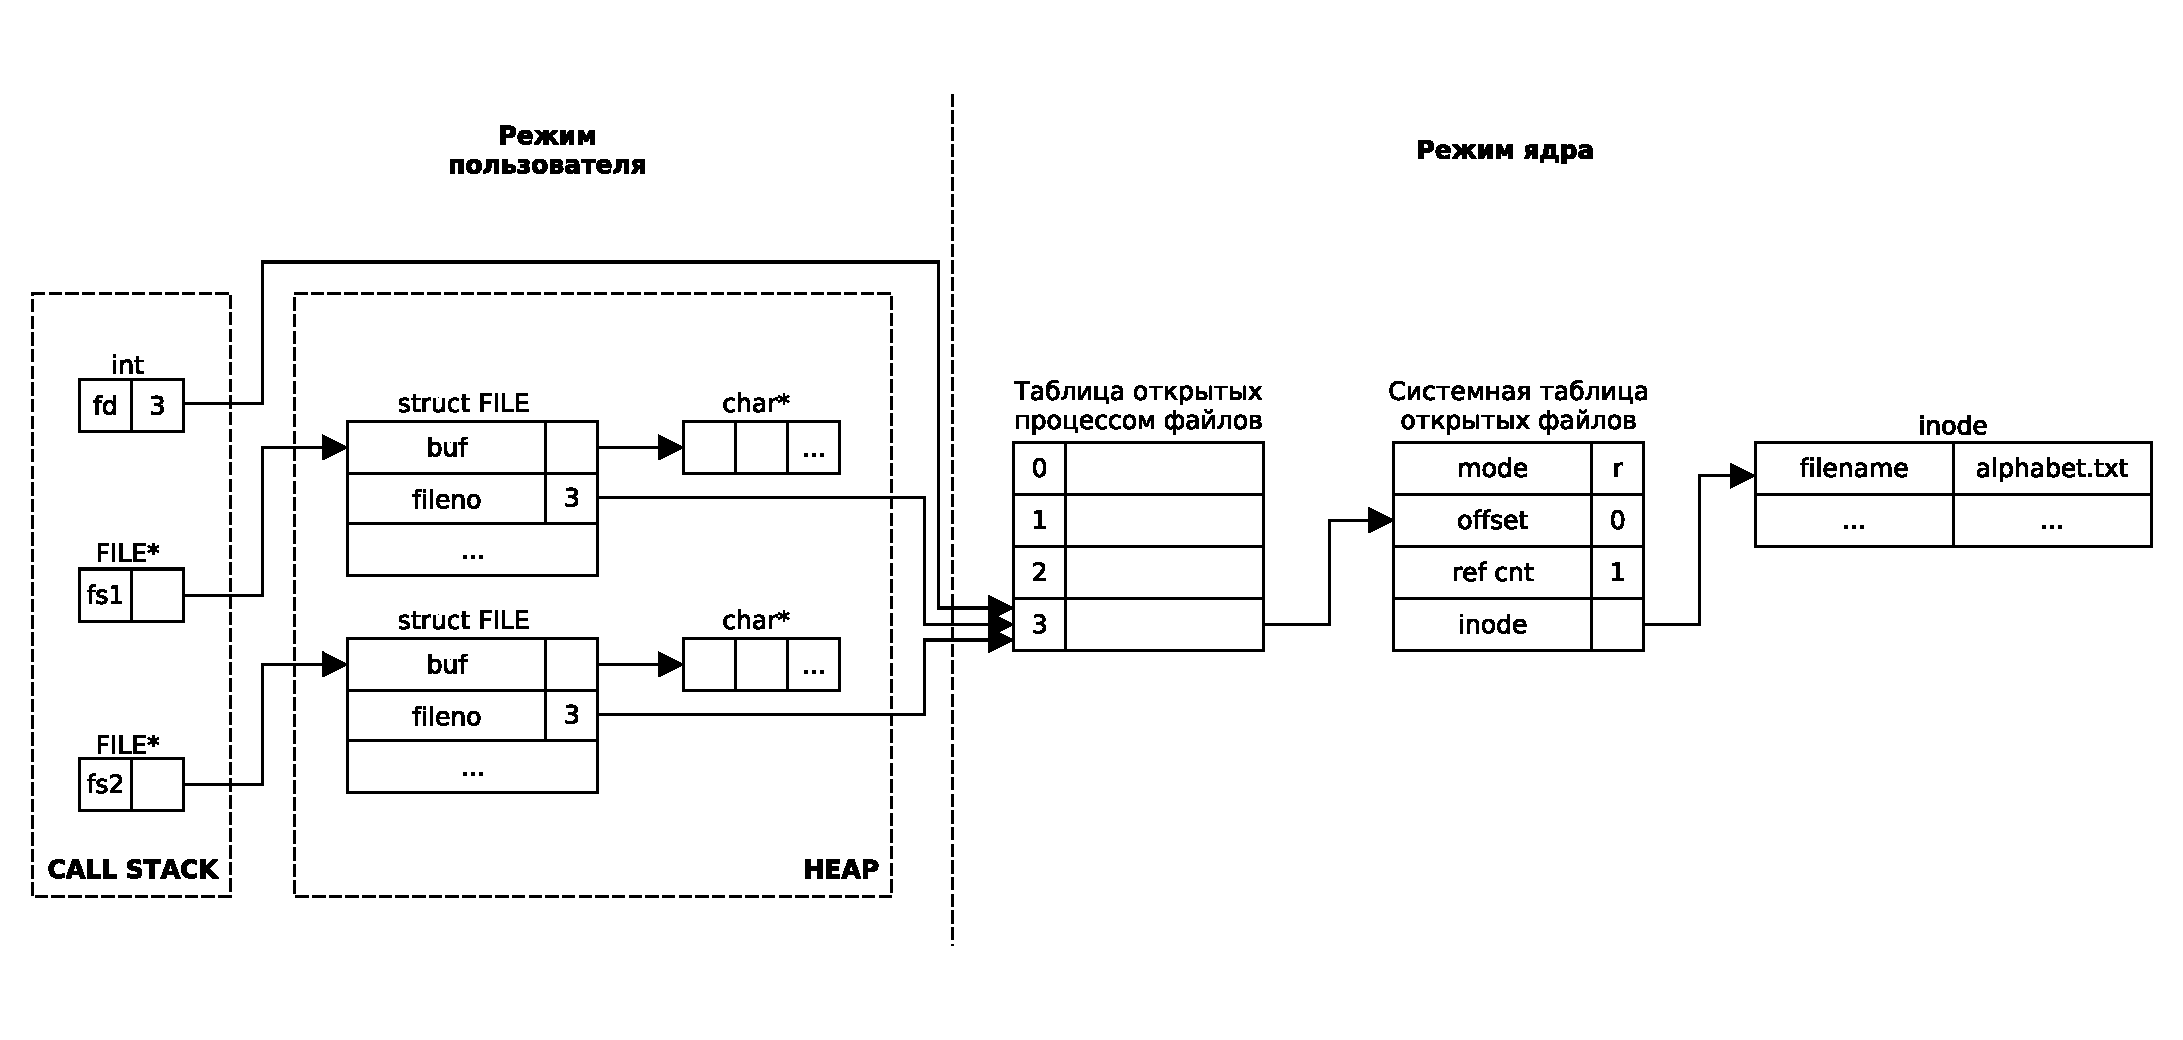
\includegraphics[scale=0.235]{images/task01.png}
    \caption{Задание \textnumero1}\label{img:task01}
\end{figure}

На рисунке~\ref{img:check01} демонстрируется, что во время выполнения процесса-сервера сокет-файл существует в файловой системе. Для этого используем команду ls с флагом -l.

\begin{figure}[H]
    \centering
    \includegraphics[scale=0.35]{images/check01.png}
    \caption{Проверка существования сокет-файла}\label{img:check01}
\end{figure}

